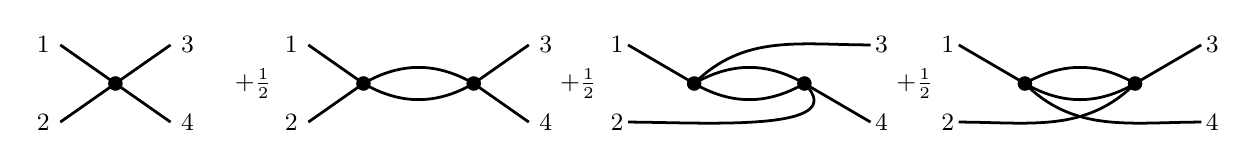
\begin{tikzpicture}[
    line width=1pt,
    every node/.style={font=\small,text=black},
    vertex/.style={draw, fill=black, circle, inner sep=1.5pt},
    extleg/.style={draw=black},
    intline/.style={draw=black},
    scale=0.7
  ]

  %--------------------------------------
  % 1) Tree‐level contact vertex at x=0
  %--------------------------------------
  \coordinate (V0) at (0,0);
  \node[vertex] at (V0) {};
  % External legs: 1 above, 2 below on left; 3 above, 4 below on right
  \draw[extleg] (V0) -- ++(-1.0,  0.7) node[left, text=black]  {1};
  \draw[extleg] (V0) -- ++(-1.0, -0.7) node[left, text=black]  {2};
  \draw[extleg] (V0) -- ++( 1.0,  0.7) node[right, text=black] {3};
  \draw[extleg] (V0) -- ++( 1.0, -0.7) node[right, text=black] {4};

  
  %--------------------------------------
  % 3) s‐channel one‐loop (at x≈4.5)
  %    • “1/2” multiplier
  %    • Two φ^4 vertices with 1,2 on left; 3,4 on right
  %--------------------------------------
  % 3a) the “1/2”
  \node at (2.5,  0) {$+ \frac{1}{2}$};

  % 3b) the s‐loop drawing
  \begin{scope}[shift={(4.5, 0)}]
    % Left φ^4 vertex
    \coordinate (Ls) at (0,0);
    \node[vertex] at (Ls) {};
    % Right φ^4 vertex
    \coordinate (Rs) at (2.0,0);
    \node[vertex] at (Rs) {};

    % External legs (no crossings in s‐channel)
    \draw[extleg] (Ls) -- ++(-1.0,  0.7) node[left, text=black]  {1};
    \draw[extleg] (Ls) -- ++(-1.0, -0.7) node[left, text=black]  {2};
    \draw[extleg] (Rs) -- ++( 1.0,  0.7) node[right, text=black] {3};
    \draw[extleg] (Rs) -- ++( 1.0, -0.7) node[right, text=black] {4};

    % Two internal propagators (forming the loop)
    \draw[intline] (Ls) to[out=30,  in=150] (Rs);
    \draw[intline] (Ls) to[out=-30, in=-150] (Rs);
  \end{scope}
  
  %--------------------------------------
  % 5) t‐channel one‐loop (at x≈9.5)
  %    • “+1/2” multiplier
  %    • External 1,2 on left; 3,4 on right but with crossings;
  %      labels moved further out
  %--------------------------------------
  % 5a) the “1/2”
  \node at (8.4, 0) {$+\frac{1}{2}$};

  % 5b) the t‐loop drawing
  \begin{scope}[shift={(10.5, 0)}]
    % Two φ^4 vertices at (0,0) and (2,0)
    \coordinate (Lt) at (0,0);
    \node[vertex] at (Lt) {};
    \coordinate (Rt) at (2,0);
    \node[vertex] at (Rt) {};

    % External node “gates” (moved farther from vertices):
    \coordinate (E1t) at (-1.2,  0.7); % 1 (left-top)
    \coordinate (E2t) at (-1.2, -0.7); % 2 (left-bottom)
    \coordinate (E3t) at (+3.2,  0.7); % 3 (right-top)
    \coordinate (E4t) at (+3.2, -0.7); % 4 (right-bottom)
    \coordinate (E1tx) at (-1.4,  0.7); % 1 (left-top)
    \coordinate (E2tx) at (-1.4, -0.7); % 2 (left-bottom)
    \coordinate (E3tx) at (+3.4,  0.7); % 3 (right-top)
    \coordinate (E4tx) at (+3.4, -0.7); % 4 (right-bottom)

    % Place labels
    \node at (E1tx) {1};
    \node at (E2tx) {2};
    \node at (E3tx) {3};
    \node at (E4tx) {4};


    % Connect 1 → Lt (straight)
    \draw[extleg] (E1t) -- (Lt);
    % Connect 3 → Lt (cross)
    \draw[extleg] (E3t) to[out=180, in=45] (Lt);
    % Connect 2 → Rt (cross under)
    \draw[extleg] (E2t) to[out=0, in=-45] (Rt);
    % Connect 4 → Rt (straight)
    \draw[extleg] (E4t) -- (Rt);

    % Two internal propagators forming the loop
    \draw[intline] (Lt) to[out=30,  in=150] (Rt);
    \draw[intline] (Lt) to[out=-30, in=-150] (Rt);
  \end{scope}

  
  %--------------------------------------
  % 7) u‐channel one‐loop (at x≈14.5)
  %    • “1/2” multiplier
  %    • External 1,2 on left; 3,4 on right with crossings;
  %      labels moved farther out
  %--------------------------------------
  % 7a) the “1/2”
  \node at (14.5, 0) {$+\frac{1}{2}$};

  % 7b) the u‐loop drawing
  \begin{scope}[shift={(16.5, 0)}]
    % Two φ^4 vertices at (0,0) and (2,0)
    \coordinate (Lu) at (0,0);
    \node[vertex] at (Lu) {};
    \coordinate (Ru) at (2,0);
    \node[vertex] at (Ru) {};

    % External node “gates”:
    \coordinate (E1u) at (-1.2,  0.7); % 1 (left-top)
    \coordinate (E2u) at (-1.2, -0.7); % 2 (left-bottom)
    \coordinate (E3u) at (+3.2,  0.7); % 3 (right-top)
    \coordinate (E4u) at (+3.2, -0.7); % 4 (right-bottom)
    \coordinate (E1ux) at (-1.4,  0.7); % 1 (left-top)
    \coordinate (E2ux) at (-1.4, -0.7); % 2 (left-bottom)
    \coordinate (E3ux) at (+3.4,  0.7); % 3 (right-top)
    \coordinate (E4ux) at (+3.4, -0.7); % 4 (right-bottom)

    % Place labels
    \node at (E1ux) {1};
    \node at (E2ux) {2};
    \node at (E3ux) {3};
    \node at (E4ux) {4};

    % Connect 1 → Lu (straight)
    \draw[extleg] (E1u) -- (Lu);
    % Connect 4 → Lu (cross back)
    \draw[extleg] (E4u) to[out=180, in=-45] (Lu);
    % Connect 2 → Ru (cross up)
    \draw[extleg] (E2u) to[out=0, in=-135] (Ru);
    % Connect 3 → Ru (straight)
    \draw[extleg] (E3u) -- (Ru);

    % Two internal propagators forming the loop
    \draw[intline] (Lu) to[out=30,  in=150] (Ru);
    \draw[intline] (Lu) to[out=-30, in=-150] (Ru);
  \end{scope}

\end{tikzpicture}
